\documentclass{beamer}
\mode <presentation>
{
    \usetheme{boxes}
    \usecolortheme{crane}
    \setbeamercovered{transparent}
}

\usepackage[absolute,overlay]{textpos}
\usepackage{pgf,pgfarrows,pgfnodes}
\usepackage[english]{babel}
\usepackage{lmodern}
\usepackage{newcent}
\usepackage{amsmath}
\usepackage{listings}
% math extension - one probably wants to use symbols like '[' (written as '$[$')
\usepackage{ucs}
%\usepackage[utf8]{inputenc}
%\usefonttheme{structuresmallcapsserif}

% utf8x does not work with xetex
\usepackage[utf8x]{inputenc}

\usepackage[normalem]{ulem}


\setlength{\TPHorizModule}{1mm}
\setlength{\TPVertModule}{1mm}
\newcommand{\WorkInProgress}{%
\begin{textblock}{14}(120.0,75.7)
\includegraphics[height=0.1cm]{./pics/rmll2011.jpg}
\end{textblock}
  }

%\setbeamercolor{background canvas}{bg=\includegraphics[width=\textwidth]{./pics/wolf.png}}

\title{FusionInventory}
\author{{FusionInventory.org}}
\subject{Assets management with FusionInventory and GLPI}
\keywords{Assets management, Inventory, FusionInventory, GLPI}

\date{Juillet 2012}
%\titlegraphic{GLPI}
%subtitle{\includegraphics[width=1.2cm]{./pics/fusioninventory-logo.png}}
\institute{\includegraphics[height=4.3cm]{./pics/rmll2011.jpg}}

\titlegraphic{}
\subtitle{RMLL 2012}
\institute{Genêve}
\author{ Walid Nouh - Mathieu Simon}
\logo{\includegraphics[height=0.7cm]{./pics/fusioninventory-logo.pdf}}

\AtBeginSection[] % Do nothing for \section*
{
    \begin{frame}<beamer>
        \frametitle{Outline}
        \tableofcontents[currentsection]
    \end{frame}
}

%%%%%%%%%%%%%%%%%%%%%%%%%%%%%%%%%%%%%%%%%%%%%%%
%%%%%%%%%%%%%%%%%%%%%%%%%%%%%%%%%%%%%%%%%%%%%%%
\begin{document}

\frame[plain]{\titlepage}


\begin{frame}
    \frametitle{About us}


    \begin{block}{Walid Nouh}
        \begin{itemize}
        \item FusionInventory contributor
        \item GLPI contributor  
        \item Work for TECLIB', Montpellier
        \end{itemize}
    \end{block}

\end{frame}

\begin{frame}
    \frametitle{About us}


    \begin{block}{Mathieu Simon}
        \begin{itemize}
        \item FusionInventory contributor
        \item 
        \item Work for , Bern
        \end{itemize}
    \end{block}

\end{frame}

\section{Project overview}

\begin{frame}
    \frametitle{From the beginning}

    \begin{description}
      \item[2006] First unified inventory agent for Unix
      \item[2008] First server implementation (Tracker, a plugin for GLPI)
      \item[2009] Agent and server integration
      \item[2010] FusionInventory project is born! 
      \item[2010] Uranos integration
      \item[2011] Rudder (cfengine) integration
      \item[2012] OTRS integration
    \end{description}

\end{frame}



\begin{frame}
    \frametitle{The project}
    %%-------------------------------------------------------------------
    %%\logo{\includegraphics[height=3.5cm]{./pics/glpi-doc.png}}
    FusionInventory is a community driven project.

    \begin{itemize}
        \item active mailing list
        \item IRC: \#FusionInventory on FreeNode
        \item Forge, Git repositories, etc
    \end{itemize}
\end{frame}


\begin{frame}
    \frametitle{Contributors}

 \begin{columns}
 \begin{column}[T]{4cm}
    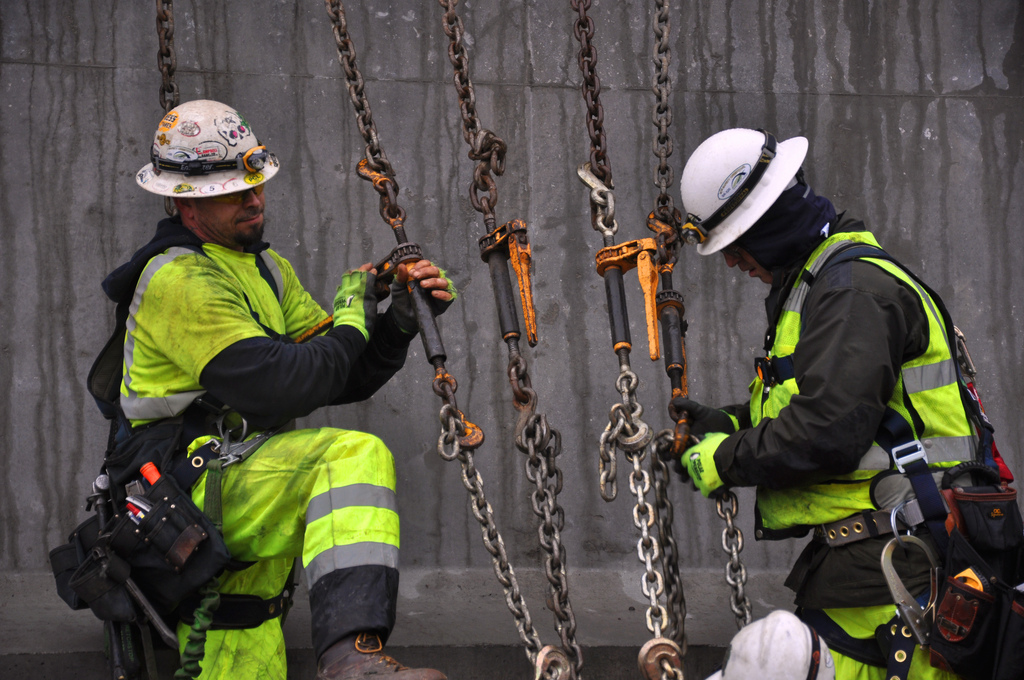
\includegraphics[height=3.7cm]{./pics/worker.jpg}
 \end{column}
 \begin{column}[t]{5cm}
    \begin{itemize}
    \item 4 active developers
    \item an active community
    \item 2 companies involved
    \end{itemize}

 \end{column}
\end{columns}

    \pause
    \bf{We're looking for more contributors !}
\end{frame}



\begin{frame}
    \frametitle{Before starting}

    \begin{block}{FusionInventory is not a software}
    \begin{itemize}
        \item Agent: a software to install on the computers
        \item Server: handles communication with the agents
        \item Task: is prepared by the server, executed by an agent
    \end{itemize}
    \end{block}

\end{frame}


\begin{frame}
    \frametitle{Available servers today}

    \begin{block}{4 solutions so far}
        \begin{itemize}
            \item FusionInventory for GLPI \\
            \url{http://www.FusionInventory.org}
            \item Uranos \\
            \url{http://uranos.sourceforge.net/}
            \item Rudder by Normation \\
            \url{http://www.normation.com/\#produits}
            \item OCS Inventory NG
            \item Mandriva Pulse 2

        \end{itemize}
        ... it's also possible to perform local XML inventory (JSON soon to come).
    \end{block}

\end{frame}

\begin{frame}
    \frametitle{In talk with}

    \begin{itemize}
    \item FusionDirectory
    \item OTRS ITSM (work already in progress)
    \end{itemize}
\end{frame}

\begin{frame}
    \frametitle{pull / push}

    \begin{block}{FusionInventory enables "push" or "pull" mode}
    \begin{itemize}
    \item \textbf{"pull": Agent $\Longrightarrow$ Server} \\
    the agent contacts the server.
    \item \textbf{"push": Agent $\Longleftarrow$ Server} \\
    the server initiate the contact.
    \end{itemize}
    \end{block}

\end{frame}

\begin{frame}
    \frametitle{Agent: Installation}


    \begin{block}{Many ways to do it}
        \begin{itemize}
            \item \textbf{distribution packages} \\
            \small{Debian, Fedora, EPEL, Ubuntu, Mageia, ...}
            \item \textbf{Windows installer} \\
            \small{GPO, psexec, ...}
            \item \textbf{static prebuilt packages}, untar and run \\
            \small{62 differents system so far}
            \item tarball and CPAN
        \end{itemize}
    \end{block}
\end{frame}

\begin{frame}
    \frametitle{Agent: Installation}

   \begin{columns}
   \begin{column}{0.35\textwidth}

\includegraphics[height=5.5cm]{pics/googleplay.png}
 \end{column}
 \begin{column}{0.65\textwidth}
There's also an Android agent available on Google Play.
 \end{column}
\end{columns}

\end{frame}


\section{Agent : target OS}

\begin{frame}
    \frametitle{Supported operating systems}

    \begin{itemize}
        \item Linux
        \item Windows
        \item MacOSX
        \item BSD
        \item AIX
        \item HP-UX
        \item Solaris
        \item Android
    \end{itemize}


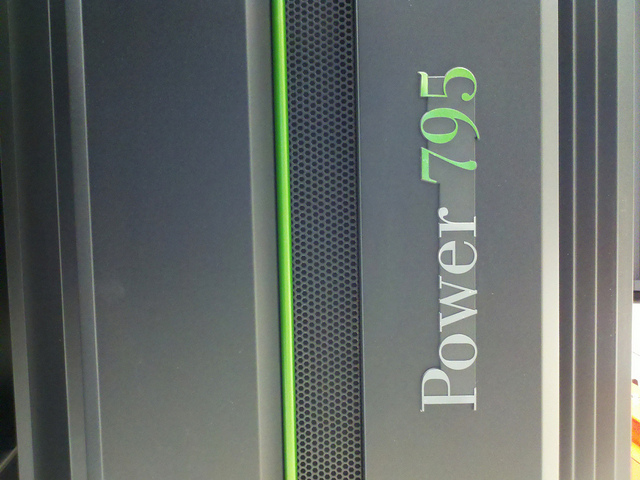
\includegraphics[height=0.5cm]{pics/logos/aix.png}
\includegraphics[height=0.5cm]{pics/logos/fedora.png}
\includegraphics[height=0.5cm]{pics/logos/hp-ux.png}
\includegraphics[height=0.5cm]{pics/logos/netbsd.png}
\includegraphics[height=0.5cm]{pics/logos/openbsd.png}

\includegraphics[height=0.5cm]{pics/logos/solaris.jpg}
\includegraphics[height=0.5cm]{pics/logos/centos.jpg}

\includegraphics[height=0.5cm]{pics/logos/linux.png}
\includegraphics[height=0.5cm]{pics/logos/osx.png}
\includegraphics[height=0.5cm]{pics/logos/ubuntu.png}
\includegraphics[height=0.5cm]{pics/logos/debian.png}
\includegraphics[height=0.5cm]{pics/logos/freebsd.png}
\includegraphics[height=0.5cm]{pics/logos/redhat.png}
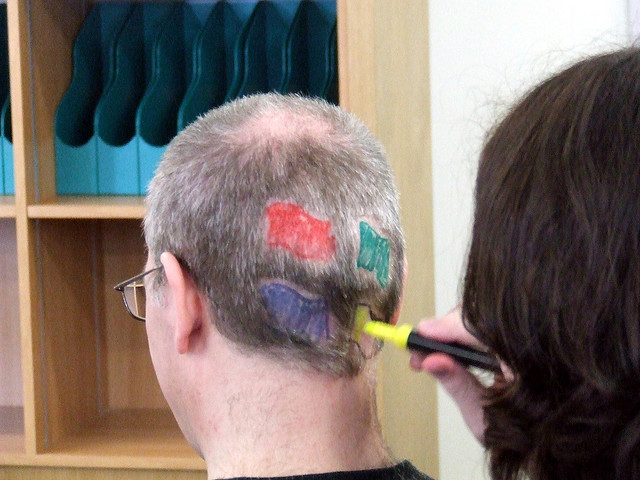
\includegraphics[height=0.5cm]{pics/logos/windows.jpg}
\includegraphics[height=0.5cm]{pics/logos/dragonflybsd.png}
\includegraphics[height=0.5cm]{pics/logos/mageia.png}

\end{frame}

\begin{frame}    
    \begin{block}{Perl helps :)}
        \begin{itemize}
            \item Few differences between Unices
            \item Also Win32...
        \end{itemize}
    \end{block}
\end{frame}

\section{Task: Network discovery}

\begin{frame}
    \frametitle{Network discovery}

    \begin{block}{Quickly collects all connected devices}
    \begin{itemize}
      \item NMAP 
      \item NetBios
      \item SNMP queries
    \end{itemize}
    \end{block}

\end{frame}

\section{Task: network inventory}
%\begin{frame}
%    \frametitle{Remote SNMP inventory}
%
%    \begin{block}{Network devices}
%        \begin{itemize}
%            \item serial number, firmware, ...
%            \item ports mapping
%        \end{itemize}
%    \end{block}
%
%    \begin{block}{Network printers}
%        \begin{itemize}
%            \item serial number, firmware, ...
%            \item cartridge ink level
%            \item page counter
%        \end{itemize}
%    \end{block}
%\end{frame}

\begin{frame}
    \frametitle{... INTERLUDE ...}

%   \begin{columns}
%   \begin{column}{0.35\textwidth}
         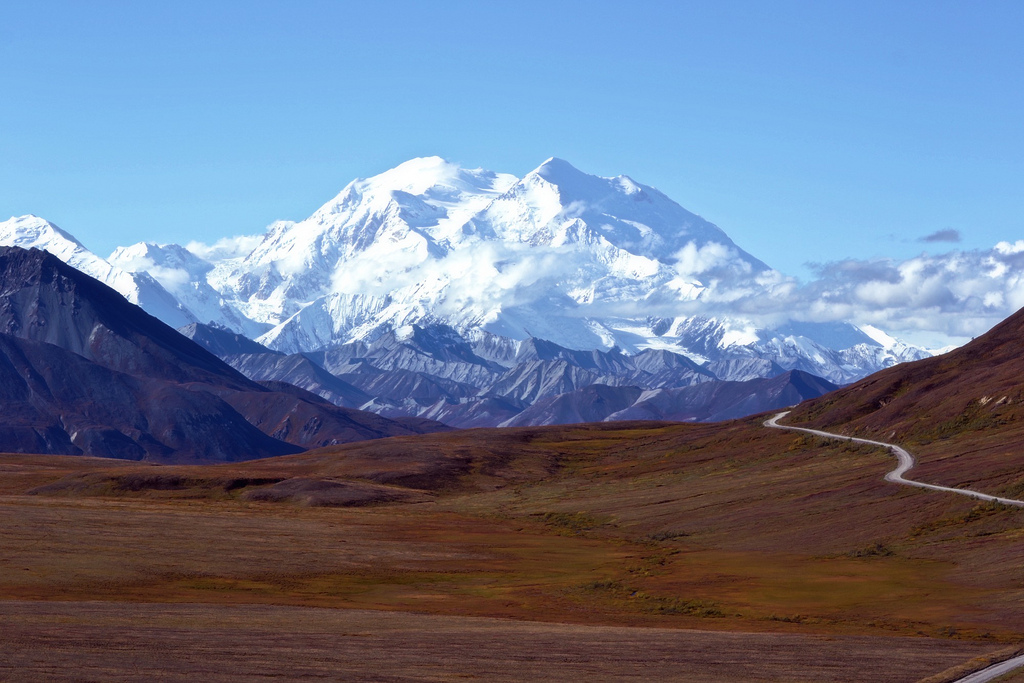
\includegraphics[height=7.5cm]{./pics/montagne.jpg}
% \end{column}
% \begin{column}{0.65\textwidth}
%    \begin{block}{... INTERM\`{E}DE ...}
%    \end{block}

% \end{column}
%\end{columns}
\end{frame}


\begin{frame}
    \frametitle{SNMP}

%    \begin{center}
%    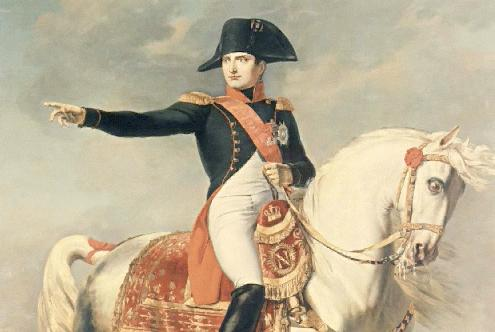
\includegraphics[height=4.0cm]{pics/napoleon.jpg}
%    \end{center}

    \begin{block}{SNMP origin}
    \begin{itemize}
    \item A standard \\
    \small{First RFC in 1988}
    \item Designed to monitor equipments
    \item 3 versions 1, 2c, 3 (Cyphering)
    \item OID: Information location
    \item MIB: A collection of OIDs
    \end{itemize}
    \end{block}
\end{frame}

\begin{frame}
    \frametitle{SNMP: what for in FusionInventory?}

    \begin{block}{How do we use SNMP?}
    \begin{itemize}
    \item Identify remote devices (network equipments, printers, ...)
    \item Perform a remote inventory
    \item Get the most important informations
    \end{itemize}
    \end{block}
\end{frame}

\begin{frame}
    \frametitle{SNMP: a nightmare}

    \begin{block}{“Please support my hardware, here is the MIB!”}

    \pause
    \begin{itemize}
    \item Might be hard to find
    \item Often no free or not redistributable 
    \item Important informations might be missing
    \item But worth, the may be wrong !
    \end{itemize}
    \end{block}

%    \begin{block}{With our SNMP models, we are sure device is well supported!}
%    \end{block}
\end{frame}
\begin{frame}
    \frametitle{SNMP: an example}

 \begin{columns}
 \begin{column}{0.35\textwidth}
         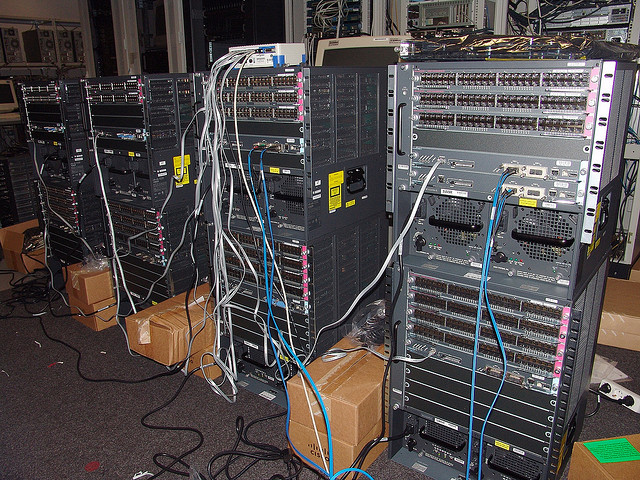
\includegraphics[height=7.5cm]{./pics/cisco.jpg}
 \end{column}
 \begin{column}{0.65\textwidth}
    \begin{block}{Example: Cisco 6500 firmware}
    12.2(33)SXI\textbf{2a} (02-Sep-09 01:00)
    \begin{itemize}
    \item Serial OID: .1.3.6.1.2.1.47.1.1.1.1.11.\textbf{1}
    \end{itemize}
    12.2(33)SXI\textbf{3} (27-Oct-09 11:12)
    \begin{itemize}
    \item Serial OID: .1.3.6.1.2.1.47.1.1.1.1.11.\textbf{2}$\Longleftarrow$ Gni?!
    \end{itemize}
    \end{block}

 \end{column}
\end{columns}


    
\end{frame}

\begin{frame}
    \frametitle{SNMP: outch}

 \begin{columns}
 \begin{column}{0.35\textwidth}
         
\includegraphics[height=7.5cm]{./pics/dead-teletubbies.jpg}
 \end{column}
 \begin{column}{0.65\textwidth}

 \end{column}
\end{columns}
\end{frame}



\begin{frame}
    \frametitle{SNMP: how to be reliable ?}

    \begin{block}{We prepared our own “MIB”}
    \begin{itemize}
    \item Manual work for each equipment
    \item stored in an XML file
    \item Defines relations between an OID and an information \\
        \small{ex: serial number → OID 1.2.4.34.53...}
    \item Supports dynamics OIDs
    \end{itemize}
    \end{block}


\end{frame}

\begin{frame}
    \frametitle{... END OF INTERLUDE ...}

    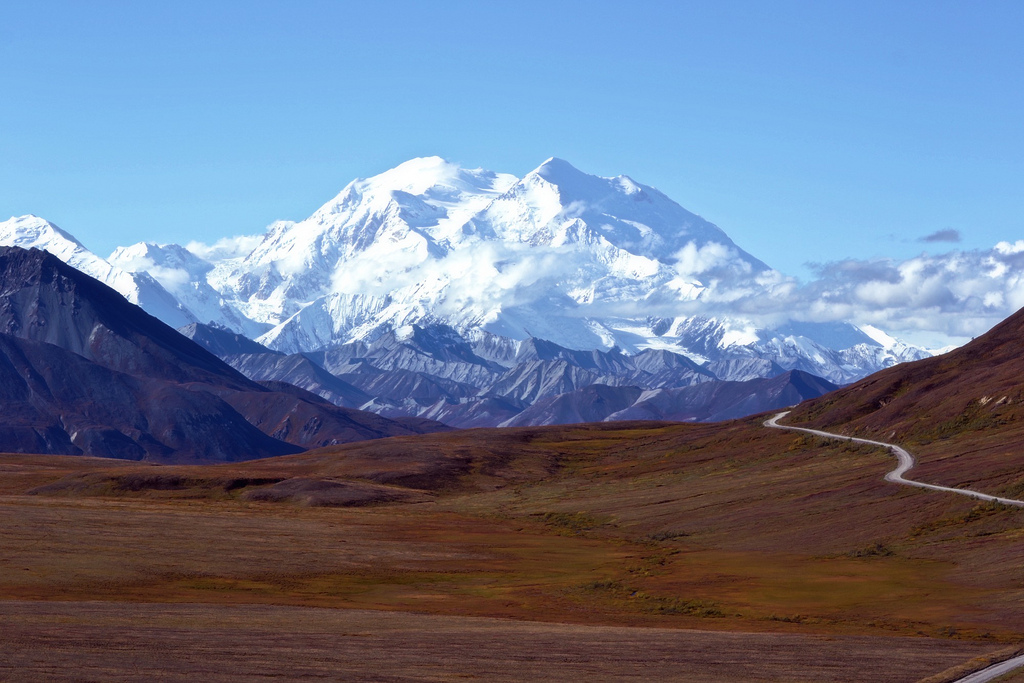
\includegraphics[height=7.5cm]{./pics/montagne.jpg}

\end{frame}



\begin{frame}
    \frametitle{SNMP: network equipments (1/3)}

    \begin{block}{Common informations}
    \begin{itemize}
    \item Serial number
    \item Supplier
    \item Model
    \item Firmware version
    \item MAC address
    \item CPU load / RAM
    \item etc
    \end{itemize}
    \end{block}
\end{frame}

\begin{frame}
    \frametitle{SNMP: network equipments (2/3)}

    \begin{block}{Advanced support}
    \begin{itemize}
    \item Number of ports
    \item Speed
    \item Internal status
    \item Errors counters
    \item VLAN
    \item Trunk (tagged)
    \item ...
    \end{itemize}
    \end{block}
\end{frame}

\begin{frame}
    \frametitle{SNMP: network equipments (3/3)}

    \begin{block}{Port to port connections}
    \begin{itemize}
    \item MAC address \\ 
    \small{one to many}
    \item LLDP / CDP discovery \\
    \small{POIP informations, etc}
    \end{itemize}
    \end{block}
\end{frame}

\begin{frame}
    \frametitle{SNMP: a network equipment example}

    \begin{center}
    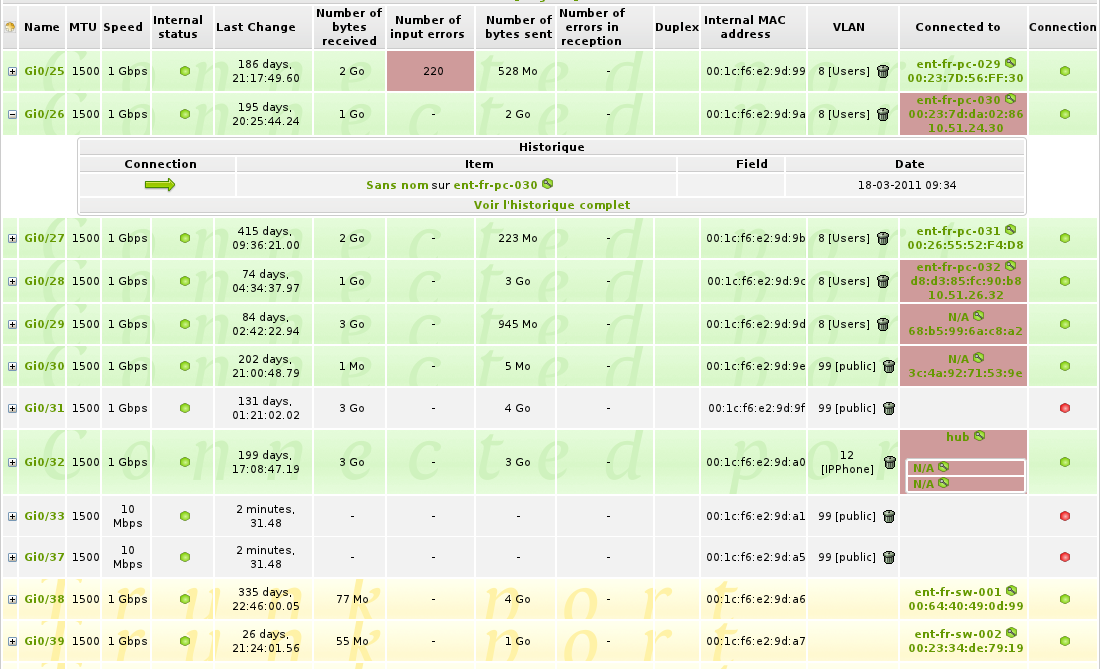
\includegraphics[width=11.7cm]{./pics/switch_ports.png}
    \end{center}
\end{frame}

\begin{frame}
    \frametitle{SNMP: Imprimante (1/2)}

    \begin{block}{Informations générales}
    \begin{itemize}
    \item Numéro de série
    \item Fabricant
    \item Modèle
    \item Firmware
    \item Mémoire
    \item Adresse MAC
    \item etc
    \end{itemize}
    \end{block}
\end{frame}

\begin{frame}
    \frametitle{SNMP: Imprimante (2/2)}

    \begin{block}{Informations avancées}
    \begin{itemize}
    \item \'{E}tats des cartouches
    \item Compteur de page
    \end{itemize}
    \end{block}
\end{frame}

\begin{frame}
    \frametitle{SNMP: exemple d'une imprimante}

    \begin{center}
    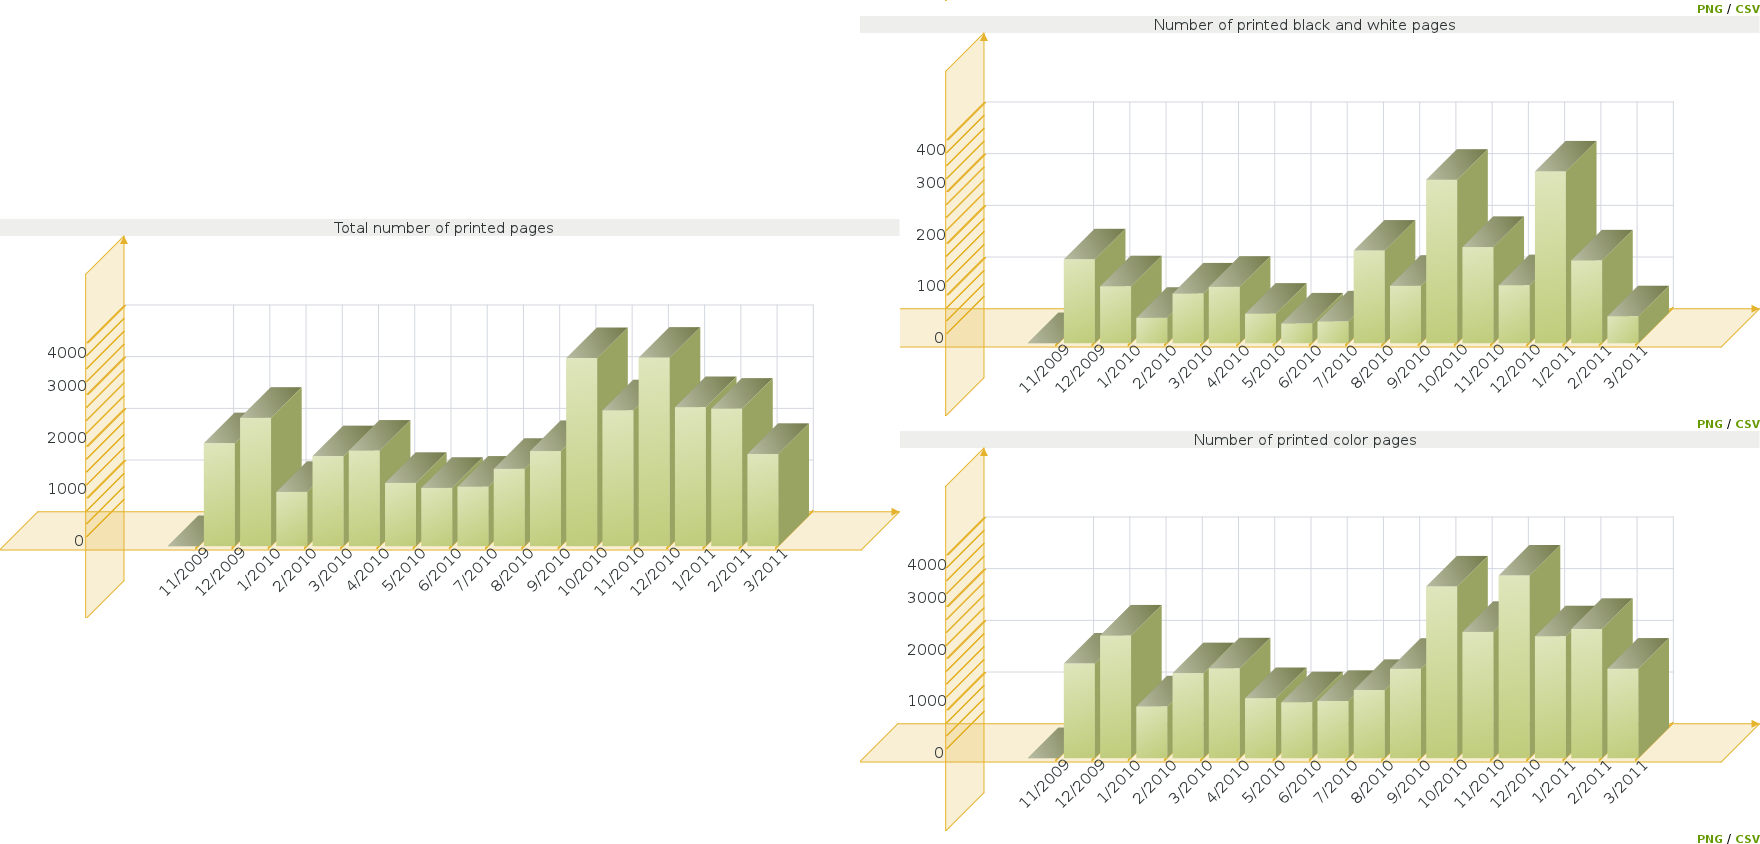
\includegraphics[width=11.7cm]{./pics/printer_graph.png}
    \end{center}
\end{frame}

\section{Tâche : Réveil sur le réseau}

\begin{frame}
    \frametitle{Wake On Lan}

    \begin{block}{WoL}
    \begin{itemize}
        \item Possiblité d'utiliser l'agent comme un proxy pour émettre des requêtes WoL.
    \end{itemize}
    \end{block}

\end{frame}

\begin{frame}
    \frametitle{Wake On Lan : Exemple}

    \begin{block}{Exemple}
    \begin{itemize}
    \item Un site distant
    \item 50 ordinateurs
    \end{itemize}
    \end{block}


    \begin{block}{Ce qu'on peut faire}
    \begin{itemize}
    \item Démarrer toutes les machines à 2h00 tous les soirs pour les mises à jour.
    \end{itemize}
    \end{block}

\end{frame}


\section{Tâche : La télédiffusion}

\begin{frame}
    \frametitle{La télédiffusion (1/2)}

    \begin{block}{Possibilité d'envoyer des actions à réaliser aux machines?}
    \begin{itemize}
        \item Pouvoir réaliser des actions sur les machines
        \item Envoyer des fichiers
        \item Réduire la bande passante grâce au “pair à pair”
    \end{itemize}
    Attention : ce n'est pas de la gestion de configuration.
    \end{block}

\WorkInProgress
\end{frame}

\begin{frame}
    \frametitle{La télédiffusion (2/2)}

    \begin{block}{Pourquoi un outil pour faire des télédiffusions vers les postes?}
    \begin{itemize}
        \item Utiliser l'interface existante de GLPI
        \item La gestion des droits de GLPI (groupes/profiles/entités)
        \item Multi-plateforme
    \end{itemize}
    \end{block}

\WorkInProgress
\end{frame}

\section{Tâche : Inventaire vCenter/ESX/ESXi}


\begin{frame}
    \frametitle{vCenter/ESX/ESXi}

    \begin{block}{Le problème}
    Des boites noires : On ne peut pas installer d'agent dessus comme pour les autres hyperviseurs.
    \end{block}


\end{frame}

\begin{frame}
    \frametitle{vCenter/ESX/ESXi}

    \begin{block}{La solution}
    L'agent peut se connecter sur les équipements VMware via l'interface SOAP API:
        \begin{itemize}
                \item inventaire Hardware
                \item lister les Machines Virtuelles
                \item lister les ESX (dans les cas des vCenter)
        \end{itemize}
    \end{block}

\end{frame}

\begin{frame}[fragile]
    \frametitle{vCenter/ESX/ESXi: en ligne de commande}

\begin{lstlisting}
fusioninventory-esx --host vcenter --user foo \ 
  --password bar --directory /tmp
\end{lstlisting}

Il ne reste plus qu'a pousser les inventaires :
\begin{lstlisting}
fusioninventory-injector -v --file /tmp/*.ocs \ 
  -u https://server/plugins/fusioninventory/
\end{lstlisting}

\end{frame}

\begin{frame}[fragile]
    \frametitle{vCenter/ESX/ESXi: l'interface GLPI}

 \begin{columns}
 \begin{column}[T]{4cm}
    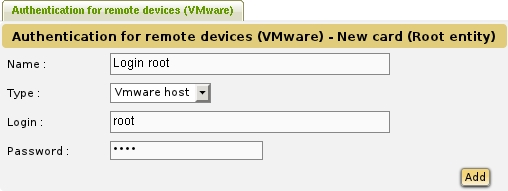
\includegraphics[height=4.0cm]{pics/esx-glpi.jpg}
 \end{column}
 \begin{column}[t]{6cm}
    \begin{block}{Une interface existe dans GLPI}
    \begin{itemize}
         \item Définir l'authentification
         \item Cibler un serveur vCenter/ESX/ESXi
         \item Planifier les inventaires
    \end{itemize}
    \end{block}
 \end{column}
\end{columns}




\end{frame}

\section{Tâche : L'inventaire}

\begin{frame}
    \begin{block}{Informations remontées (1/3)}
        \begin{itemize}
        \item BIOS
        \item modules PCI
        \item slots mémoires
        \item CPUs
        \item disques durs, lecteur, etc
        \item carte mère
        \item système d'exploitation
        \item écrans
        \item ports
        \item slots
        \item partitions
        \item logiciels
        \end{itemize}
    \end{block}
\end{frame}

\begin{frame}
    \begin{block}{Informations remontées (2/3)}
        \begin{itemize}
        \item utilisateurs connectés
        \item cartes vidéos
        \item machines virtuelles
        \item carte sons
        \item modems
        \item variables d'environnement
        \item équipements USB
        \item configuration réseau
        \item batteries
        \item imprimantes
        \item processus
        \item antivirus
        \item LVM
        \end{itemize}
    \end{block}
\end{frame}

\begin{frame}
    \begin{block}{Informations remontées (3/3)}
        Android: carte SIM, IMEI , etc
    \end{block}
\end{frame}

\section{La qualitaï!}

\begin{frame}
    \frametitle{Quelques métriques}

    \begin{block}{Aujourd'hui}
        \begin{itemize}
            \item 194 modules Perl
            \item 21851 lignes
            \item 938 tests unitaires
        \end{itemize}
    \end{block}

\end{frame}


\begin{frame}
    \frametitle{Quelques métriques}

    \begin{block}{Aujourd'hui}
        \begin{itemize}
            \item 194 modules Perl
            \item 21851 lignes
            \item \bf{938 tests unitaires} !
        \end{itemize}
    \end{block}

\end{frame}

\begin{frame}
    \frametitle{test-unitaire}

    \begin{block}{Pour ?}
        \begin{itemize}
            \item tester le parsing sur des OS qu'on a pas
            \item vérifier le code Win32 depuis un autre OS \\
            \small{jusqu'a WMI et la base de registre}
            \item vérifier des choses pénibles \\
            \small{unicode, HTTPS, etc}
        \end{itemize}
    \end{block}

\end{frame}

\section{D'un point de vu développeur}

\begin{frame}
    \frametitle{Ce que FusionInventory peut apporter}

    \begin{block}{Plusieurs scénarii}
        \begin{itemize}
            \item Utiliser l'inventaire dans votre application
            \item Etendre la couverture de l'inventaire
            \item Interface avec GLPI ou autres \\
            \small{Uranos, bientôt OTRS, etc}
            \item Créer des nouvelles tâches
        \end{itemize}
    \end{block}

\end{frame}

\begin{frame}

    \begin{block}{Utiliser l'inventaire dans votre application}
    demo
    \end{block}

\end{frame}


\begin{frame}

    \begin{block}{Etendre la couverture de l'inventaire}
    demo
    \end{block}

\end{frame}

\begin{frame}

    \begin{block}{Créer des nouvelles tâches}
    Vous permet de récuperer facilement des objets dans le bon contexte :
    \begin{itemize}
      \item \$serveur
      \item \$config
      \item \$logger 
    \end{itemize}
    \end{block}

\end{frame}

\begin{frame}

    \begin{block}{Interface avec GLPI ou autres}
        \begin{itemize}
            \item SOAP (GLPI et OTRS)
        \end{itemize}
    \end{block}

\end{frame}

\section{La suite}

\begin{frame}
    \frametitle{What else?}

    \begin{center}
    \includegraphics[height=4.0cm]{pics/whatelse.jpg}
    \end{center}

\end{frame}

\begin{frame}
    \frametitle{Notre roadmap}

    Prochaines étapes :
    \begin{itemize}
        \item FusionInventory Agent 2.3.x
        \item \'{E}diteur de modèle SNMP XML
        \item Intégration avec nut 
    \end{itemize}

    Transition en cours :
    \begin{itemize}
        \item OCS/XML → REST/JSON
        \small{prévue pour l'agent 3.0.0\\utilisée par OTRS}
    \end{itemize}

\end{frame}


\section{Questions}

\begin{frame}
    \frametitle{Questions?}

%    \bf{Questions?}
    \begin{center}

    \includegraphics[height=5cm]{./pics/question.pdf}

    \end{center}
%    \includegraphics[height=7.5cm]{./pics/ask.jpg}

\end{frame}

\begin{frame}
    \frametitle{Thanks}

    \begin{block}{Thanks!}
        \begin{itemize}
            \item Windows \url{http://www.flickr.com/photos/aeu04117/430338509/sizes/z/in/photostream/}
            \item AIX \url{http://www.flickr.com/photos/pchow98/5115638572/}
            \item MacOSX \url{http://www.flickr.com/photos/adriannier/5555516312/sizes/l/in/photostream/}
            \item Cisco 6500 \url{http://www.flickr.com/photos/joachim\_s\_mueller/3084164647/sizes/z/in/photostream/}
            \item Teletubbies \url{http://www.flickr.com/photos/tudor/232849285/lightbox/}
            \item Worker \url{http://www.flickr.com/photos/wsdot/6783674428/sizes/l/in/photostream/}
            \item Bee \url{http://www.flickr.com/photos/8583446@N05/7454903214/sizes/l/in/photostream/}
            \item Montagne \url{http://www.flickr.com/photos/blmiers2/6167391543/sizes/l/in/photostream/} 
        \end{itemize}
    \end{block}
\end{frame}




\end{document}
